We analyze four different ML domains to showcase trade-offs in preprocessing pipeline optimizations: CV, NLP, {\color{diff}Audio}, and non-intrusive load monitoring (NILM).
{\color{diff}We evaluate the pipelines with in total seven different datasets in order to compare the impact of different encodings and image resolutions on the respective pipeline's performance.}
Every pipeline is based on common preprocessing steps from popular models and datasets in their respective domains.
We assume that the training throughput is unbounded for our analysis, as we are interested in maximizing $T_4$ irrespective of the actual model.
This section showcases the design of our profiling library, the individual pipelines and defines the experimental setup.

\subsection{PRESTO Library}

After initial manual profiling attempts, we decided to create the \textbf{Pre}processing \textbf{St}rategy \textbf{O}ptimizer (PRESTO) library that automates the generic pipeline profiling process.
The library can be used with any preprocessing pipeline written with the TensorFlow \texttt{tf.data} API~\cite{murray2021tf}, and hence, is readily applicable to different use cases.

PRESTO contains a \texttt{Strategy} wrapper class that splits the preprocessing pipeline at any given step into an offline and online part.
This is done by inserting a serialization and loading step at the \textit{split position} with the TFRecord format, a wrapper around the Protobuf encoding~\cite{protobuf} for TensorFlow.
Additional parameters include the parallelism, sharding, {\color{diff}caching behavior, and compression format}, as well as the temporary logging directory.

%\vspace{-0.2cm}
% \begin{figure}
%   \centering
%   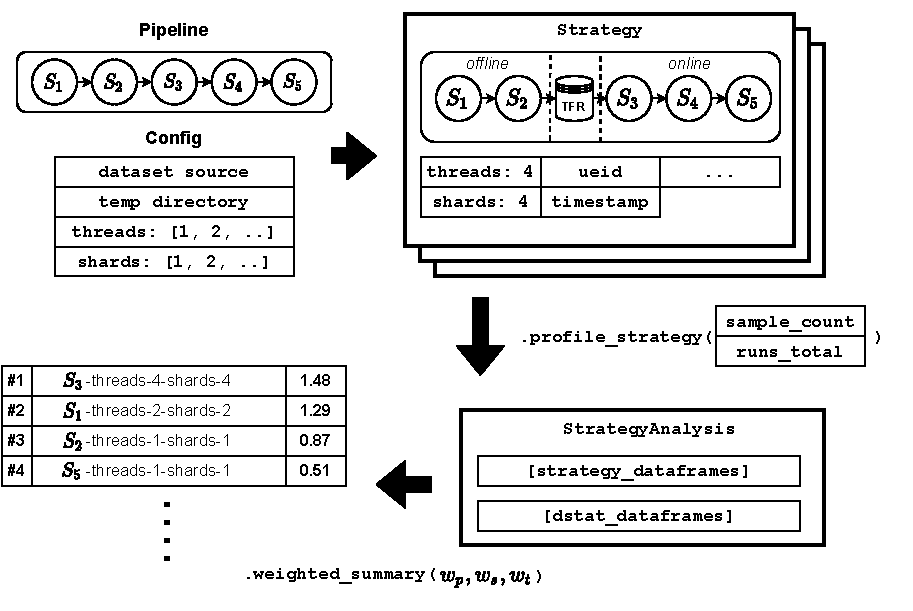
\includegraphics[width=0.47\textwidth]{figures/misc/pbr-prototype-diagram.pdf}
%   \caption{PRESTO library design}
%   \label{fig:prototype}
% \end{figure}
%\vspace{-0.3cm}
The strategy wrapper class executes the entire preprocessing pipeline through the \texttt{tf.data} API.
We simulate the training process by accessing the sample tensor's shape member to measure the preprocessing throughput without training an actual model. 
This allows us to profile the preprocessing pipeline's throughput by calling the \texttt{profile\_strategy()} function.
It accepts two parameters which have to be set manually: \texttt{sample\_count} and \texttt{runs\_total}.
{\color{diff} While it is useful to get an initial understanding of a pipeline's performance with less samples, some bottlenecks only show after local caches are full or a network link is used to its maximum capacity, so that we recommend profiling with the entire dataset.}
%Both parameters affect the amount of time used for the complete profiling, as every additional run usually adds a constant factor. An increased amount of samples can trigger a bottleneck which may slow down the experiments considerably. 

Profiling focuses on three key metrics - \textit{preprocessing time}, \textit{storage consumption} and \textit{throughput} - which can be easily tracked by internal Python code.
For more in-depth information, \texttt{dstat} is executed in parallel and provides specific system-level information, like disk read/write loads and network traffic in case of network storage.
These stats and additional metadata, like a unique hash and the split position, are returned as Pandas dataframes~\cite{mckinney-proc-scipy-2010}.

After the profiling is finished, the \texttt{StrategyAnalysis} class summarizes the findings and provides a semi-automatic way to pick the best strategy based on {\color{diff}an objective function.}
The function normalizes the individual metrics to the range of $[0, 1]$ based on their minimum and maximum values and multiplies them by user-defined weights $w_{p, s, t}$.
Let preprocessing time be $\textbf{p}$, storage consumption $\textbf{s}$, and throughput $\textbf{t}$ as vectors of the respective values for all strategies:
\begin{align*}
    f(w_p, w_s, w_t, \textbf{p}, \textbf{s}, \textbf{t}) = w_p \times |\textbf{p}| + w_s \times |\textbf{s}| + w_t \times |\textbf{t}|
\end{align*}
{\color{diff}
The weights $w_{p, s, t}$ are can be defined manually, based on the user's objective.}
As an example, we want to find the optimal strategy to apply hyperparameter tuning on a model before a deadline.
That means we want a low preprocessing time and the highest possible throughput, while the storage consumption is irrelevant. In this case, the weights would look as follows:
\begin{align*}
(w_p, w_s, w_t) = (1,\; 0,\; 1)
\end{align*}
{\color{diff}
On the contrary, if we have access to a cluster with a lot of compute power and are not in a race against time, it will be preferable to sort only by throughput $(w_{p,s} = 0, w_t = 1)$, which is a good default configuration.}
{\color{diff}This procedure can be applied to every strategy, which can have different parallelization, sharding and compression options and lead to new trade-offs.}
{\color{diff}More complex objective functions} can feature cloud providers' processing and storage prices.
We presume that renting a low-cost VM and profiling the different strategies could probe the infrastructure, i.e., network bandwidths.
This allows us to extrapolate the processing performance by tensor-specific CPU benchmarks like PASTA~\cite{li2020parallel} for high-cost VMs.
We provide our library as an open-source project at \href{https://github.com/cirquit/presto}{https://github.com/cirquit/presto}.

\vspace{-0.2cm}
\subsection{Pipelines}

We profiled {\color{diff}seven} pipelines from four different domains and designed them to represent popular DL models.
Table~\ref{tab:experiments:dataset-info} shows the seven datasets we used to profile the pipelines with their storage consumption, sample count, and format.
The datasets and pipelines show a variety of common formats, and different intermediate sizes, e.g., the NLP pipeline has a strategy that increases the initial storage consumption by $64\times$, while NILM has a strategy that decreases the initial storage consumption by a factor of $12\times$ (Fig.~\ref{fig:ss-vs-thr}).
The pipelines were implemented with the \texttt{tf.data} API~\cite{murray2021tf} which automates pipeline execution and allows us to parallelize computations easily.
We define a \textit{sample} in this context as data that is used as input for a DL model.

{\color{diff}The naming of the steps in the pipelines follows a common pattern.
First, the data is read from disk (\texttt{unprocessed}).
After reading the dataset from disk, a concatenation step transforms the input files into a single TFRecord binary in order to allow for efficient sequential read access (\texttt{concatenated}).
The concatenation step was technically not feasible for the Audio pipeline, and was omitted for the NILM pipeline as the raw data was already stored in concatenated binary form.
Then, the data is decoded into a tensor format (\texttt{decoded}).
}
{\color{diff3}
Finally, additional transformation steps can be applied to bring the data into a format suitable for the training process.
Generally, the steps have two characteristics: the online processing time and the relative increase or decrease of storage consumption.
We explain the trade-off between these two characteristics in Sec.~\ref{ssec:storage-versus-throughput}, which can change for the same step just by using different datasets, e.g., decoding can increase or decrease the storage consumption depending on the initial file encoding (e.g., JPG vs. PNG).

The performance of preprocessing steps depends not only on the implementation of the step itself, but also on its position in the pipeline and on the input data. We specifically showcase this behaviour in Sec.~\ref{ssec:modifying-pipeline} by changing the position of a new step in an existing profiled pipeline.
}

%The only exception is the high-frequency dataset CREAM, where one has to aggregate a raw electrical signal to make it usable in a model; hence, the storage consumption per sample is considerably higher.
\vspace{-0.5cm}
\begin{table}[h]
\scalebox{0.7}{
\begin{tabular}{llrrrl}
\textbf{Dataset} & {\color{diff}\textbf{Pipeline}} & \thead{Sample\\ Count} & \textbf{Size in GB} & \thead{Avg. Sample\\ Size in MB} & \textbf{Format} \\ \hline
ILSVRC2012~\cite{ILSVRC15} & {\color{diff}CV} & 1.3M & 146.90 & 0.1147 & JPG \\ \hline
{\color{diff}Cube++ JPG~\cite{ershov2020cube}} & {\color{diff}CV2-JPG} & 4890 & 2.54 & 0.5203 & JPG \\ \hline
{\color{diff}Cube++ PNG~\cite{ershov2020cube}} & {\color{diff}CV2-PNG} & 4890 & 85.17 & 17.4176 & PNG  \\ \hline
OpenWebText~\cite{Gokaslan2019OpenWeb} & {\color{diff}NLP} & 181K & 7.71 & 0.0427 & TXT \\ \hline
CREAM~\cite{jorde2020cream} & {\color{diff}NILM} & 268K & 39.56 & 0.1477 & HDF5 \\ \hline
Commonvoice (en)~\cite{ardila2019common}  & {\color{diff}MP3} & 13K & 0.25 & 0.0197 & MP3 \\ \hline
Librispeech~\cite{panayotov2015librispeech} & {\color{diff}FLAC} & 29K & 6.61 & 0.2319 & FLAC
\end{tabular}
}
\caption{Metadata of all profiled datasets.}
\label{tab:experiments:dataset-info}
\end{table}
\vspace{-0.8cm}

\subsubsection{CV}

{\color{diff}We profile three datasets with the CV pipeline (Fig.~\ref{fig:cv-pipeline}) to analyze the performance under different image resolutions and encodings. 
ILSVRC2012~\cite{ILSVRC15} is a low resolution, JPG encoded subset of ImageNet~\cite{deng2009imagenet} and is a popular and commonly acknowledged dataset for visual object recognition.
Cube++ is a high-resolution dataset and comes in two flavors: as 16-bit encoded PNGs and JPGs~\cite{ershov2020cube}.
The difference in storage consumption between the two encodings allows for a direct comparison of the decoding performance.
The images from Cube++ are roughly $5\times$ larger than in ILSVRC2012, which allows to analyze how much the image resolution affects the throughput of each strategy.}
Details of this pipeline have been discussed in Section~\ref{sec:introduction}.
%An additional augmentation strategy, \textit{random-cropped} is added to the preprocessing pipeline after the last strategy.
%As this augmentation is not deterministic, it must be performed online and can not be used as a split position.

\subsubsection{NLP}

The NLP pipeline  (Fig.~\ref{fig:nlp-pipeline}) is based on GPT-2~\cite{radford2019better}, a popular transformer-based model which tries to predict the next word based on the textual input.
We used the dataset from the corresponding open-source implementation~\cite{Gokaslan2019OpenWeb} of OpenWebText, which was replicated from the GPT-2 paper.
Our version of the dataset is an early iteration and takes up 8\:GB compared to the most current one at 12\:GB.
The dataset consists of HTML content from scraped URLs that have been upvoted on Reddit, a social media platform, as an indicator of human interest and intelligible content. It is stored as multiple text files.

The preprocessing starts with reading text files ({\color{diff}\texttt{concatenated}}) and decoding the actual textual content ({\color{diff}\texttt{decoded}}) with the same HTML parsing library (newspaper~\cite{newspaper2020}) as GPT-2.
Each word is encoded into an \texttt{int32} via Byte Pair Encoding~\cite{DBLP:journals/corr/SennrichHB15} ({\color{diff}\texttt{bpe-encoded}}), which is then looked up in a word2vec embedding~\cite{mikolov2013efficient} that returns a \texttt{float32} tensor of dimension $1\times768$ ({\color{diff}\texttt{embedded}}).
This vector is stacked for every word in the text, resulting in an $n\:\times\:768$ tensor, the final model input.
These preprocessing steps' complexity depends on the tokenization model and the final embedding, making their performance hard to predict.

\vspace{-0.1cm}
\begin{figure}[h]
    \centering
    \begin{subfigure}[b]{0.38\textwidth}
        \centering
        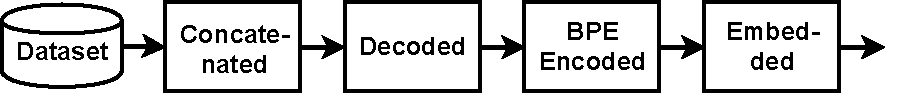
\includegraphics[width=\textwidth]{figures/openwebtext-pipeline/pipeline.pdf}
        \caption[]%
        {{\small NLP }}    
        \label{fig:nlp-pipeline}
    \end{subfigure}
    \hfill
    \begin{subfigure}[b]{0.23\textwidth}  
        \centering 
        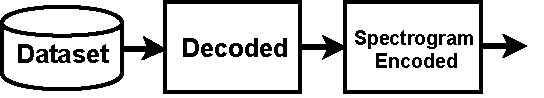
\includegraphics[width=\textwidth]{figures/commonvoice-pipeline/pipeline.pdf}
        \caption[]%
        {{\small MP3 + FLAC}}    
        \label{fig:audio-pipeline}
    \end{subfigure}
    \hfill
    \begin{subfigure}[b]{0.23\textwidth}   
        \centering 
        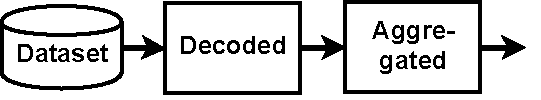
\includegraphics[width=\textwidth]{figures/cream-pipeline/pipeline.pdf}
        \caption[]%
        {{\small NILM }}    
        \label{fig:cream-pipeline}
    \end{subfigure}
    \vspace*{-0.3cm}
    \caption[]
    {\small Preprocessing pipelines} 
    \label{fig:all-pipelines}
\end{figure}
\vspace{-0.45cm}

\subsubsection{Audio Processing}

For the audio pipelines, we took inspiration from Baidu's Deep Speech model~\cite{hannun2014deep, amodei2016deep}.
Deep Speech is an RNN-based model that translates spoken audio samples to text.
Both preprocessing pipelines (Fig.~\ref{fig:audio-pipeline}) decode the compressed audio signal into the raw waveform ({\color{diff}\texttt{decoded}}) of the size $l \times r$, where $l$ is the sample duration in seconds and $r$ is the sampling rate encoded as \texttt{int16}.
The waveform is transformed using a short-time Fourier transform (STFT) with a window size of 20\:ms and a stride of 10\:ms.
The spectrogram is then transformed using an 80-bin mel-scale filter bank, leading to a size $\frac{l - 20ms + 10ms}{10ms} \times 80$ tensor encoded as \texttt{float32} ({\color{diff}\texttt{spectrogram-encoded}}).
The difference between the pipelines is their respective input format (MP3 vs. FLAC).
In contrast to some implementations~\cite{hannun2014deep}, we do not convert the data to mel-frequency cepstral coefficients (MFCCs) because it has been found that DL models work as well or better without this transformation~\cite{huzaifah2017comparison, purwins2019deep, solovyev2020deep}.

As datasets, we use the Mozilla Commonvoice 5.1 English corpus~\cite{ardila2019common} for MP3 files and the Librispeech dataset~\cite{panayotov2015librispeech} for FLAC files.

\subsubsection{NILM}

Our signal processing pipeline is based on MEED~\cite{jorde2019meed}, a state-of-the-art event detection model used for non-intrusive load monitoring of electrical data.
The task is to classify individual appliances based on the aggregated voltage and current reading measured on a building's mains.
These datasets typically have a very high frequency, e.g., 6,400-50,000\;Hz~\cite{anderson2012blued, kriechbaumer2018blond, jorde2020cream} to provide information on subtle changes that can be useful for appliance identification.

We used CREAM~\cite{jorde2020cream}, a component-level electrical measurement dataset for two industrial-grade coffeemakers encoded as HDF5 files per hour.
CREAM contains two datasets from two different coffee machines (X8 and X9), from which we used the larger X8 dataset because it takes up more than double the storage consumption of X9, i.e., totals 744 hours of 6.4\:kHz sampled current and voltage.
This dataset's fundamental difference to the other datasets is the \texttt{float64} encoding, which is favorable for NILM tasks~\cite{kahl2017comprehensive} but introduces additional storage consumption.

The pipeline starts by reading HDF5 files and extracts the voltage and current signals from them {\color{diff}(\texttt{decoded})}. They are sliced in 10-second windows, which results in a $2\times64.000$ tensor of \texttt{float64}.
Then, three aggregated values are computed: the reactive power~\cite{barsim2014unsupervised}, the root-mean-square of the current, and its cumulative sum~\cite{jorde2019meed, trung2014event, zhu2018novel} ({\color{diff}\texttt{aggregated}}). 
These aggregation operators work with a dataset period length of 128, which results in a tensor of size $3\times500$ encoded as \texttt{float64}.

%\vspace{-0.2cm}
\subsection{Experimental Setup}
\label{ssec:experimental-setup}

We execute our experiments on a virtual machine with {\color{diff}80\:GB} DDR4 RAM, 8\:VCPUs on an Intel Xeon E5-2630 v3 8x@2.4\:GHz with an Ubuntu 18.04 image on our OpenStack cluster.
Our Ceph cluster, {\color{diff}backed by HDDs}, is used as a storage device via \textit{cephfs}, with a $10$\:Gb/s uplink and downlink.
This storage is used for both storing the intermediate dataset representations as well as the unprocessed datasets.
We repeat each experiment five times and we drop the page cache after every run to remove memory caching effects {\color{diff}except for explicitly marked caching experiments.
All experiments are run with 8 threads except for explicitly marked scalability experiments with a sharded dataset so that every thread has an assigned individual file to read in parallel.}
All experiments are executed with Python 3.7 and TensorFlow 2.4.
Specific library versions are available in our GitHub repository.